\documentclass[portrait,paperwidth=91cm,paperheight=121cm,fontscale=0.35]{baposter} % 48x36 inch paper

\usepackage[utf8]{inputenc}



\begin{document}

\begin{poster}{columns=3, background=none}

{Dependable Interference-Aware Time-Slotted Channel Hopping for Wireless Sensor Networks}
{Ankita Upadhyay   (aaupadhy@ucsc.edu)\\University of California, Santa Cruz}

\headerbox{Introduction}{name=introduction, column=0}
{ Time-Slotted Channel Hopping (TSCH)'s main goal is to ameliorate communication reliability in Wireless Sensor Networks (WSNs). This is accomplished by reducing the medium access contention (MAC) impact. Elements that comprise the MAC impact include blocking of wireless links and multi-path fading. TSCH performs better than single-channel communications. For instance, in-vehicle networks include interference which is dynamic and leads to non-guaranteed reliability throughout time. This poster depicts an Enhanced version of the TSCH protocol together with a Distributed Channel Sensing technique (ETSCH+DCS) which aims to detects good quality channels to be utilized for communication. The channel quality is extracted using a distributed channel-quality estimation technique. The central technique uses a Non-Intrusive Channel-quality Estimation (NICE) technique that detects energy interference in each timeslot's idle parts at the network coordinator location. 
}

f
\headerbox{Results}{name=results, column=0, below=introduction}
{Figure 4 shows the distribution
of average PRR of all links in the network over a window of 500 transmissions for the different
mechanisms and scenarios. The results show that using an (Enhanced Beacon Slotted List) EBSL generally leads to a lower standard
deviation in the PRR results. This guarantees a higher reliability level for the links of the network.
Figure 7(a) shows that for the scenario with no controlled noise generator, the standard deviation
of ETSCH–EBSL results is higher than for TSCH. This is because TSCH always uses the same HSL
for hopping, while ETSCH–EBSL may use different sets of channels as the HSL due to detecting low
noise on some channels.
 
     \centering
     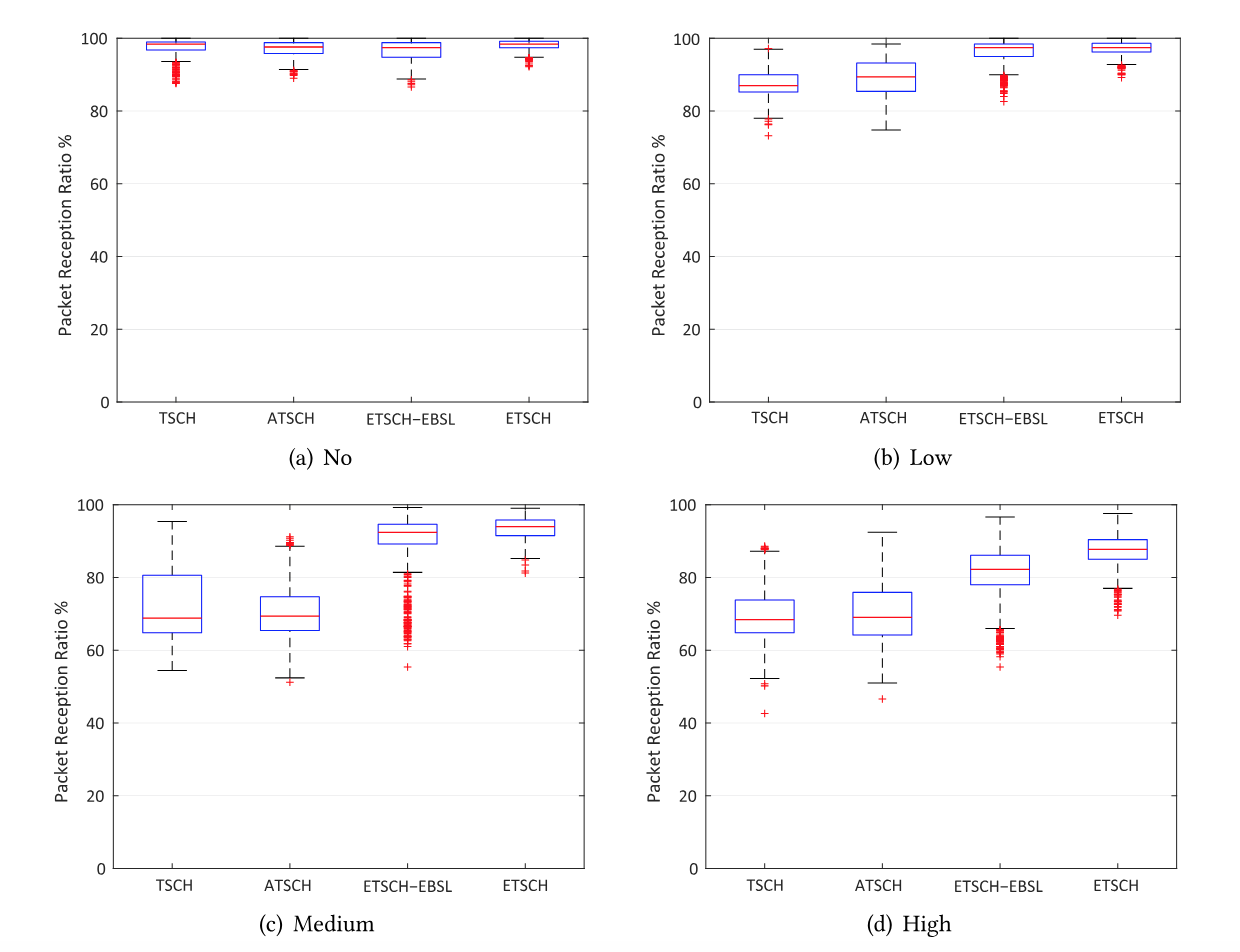
\includegraphics[height=6.5cm, width=\textwidth]{fourgraphs1.png}
      \caption{Figure 4: PRR distribution of all network links, over a window of 500 transmissions}

      \centering
      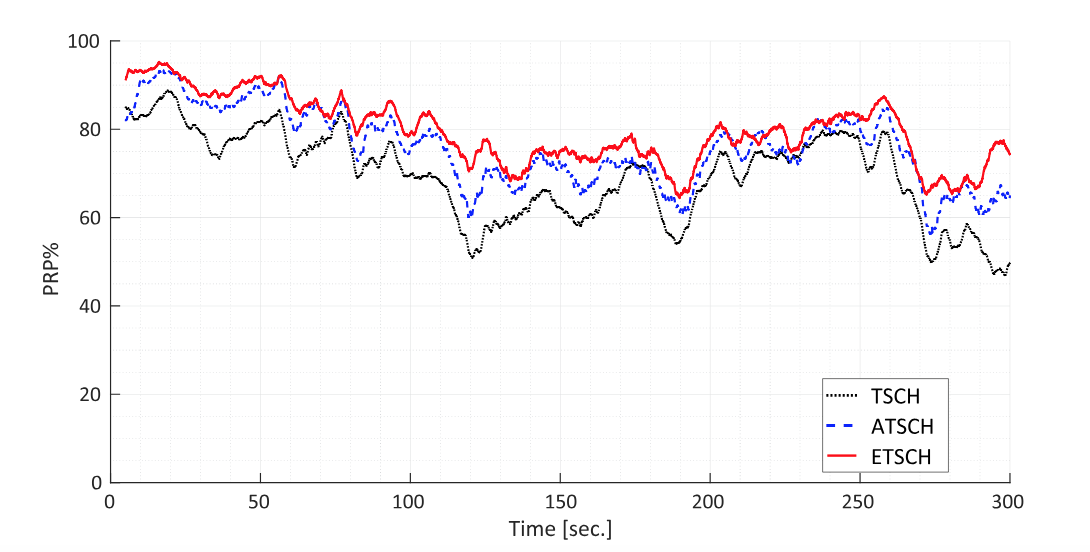
\includegraphics[height=5.7cm, width=\textwidth]{redblue.png}
      \caption{Figure 5: Effect of the Mixed lifelike interference }
      
      \centering
      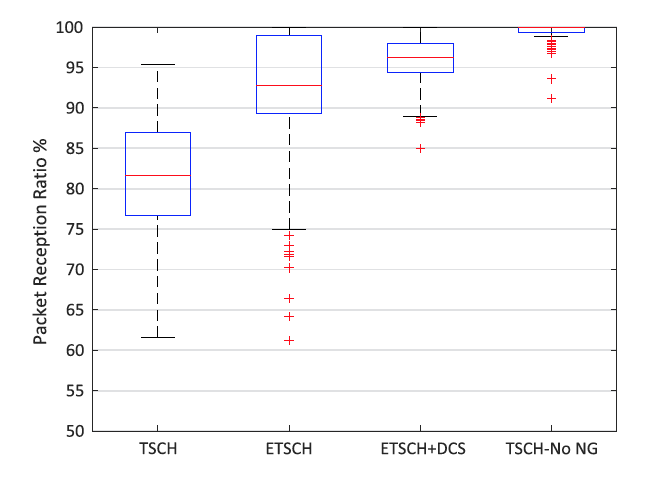
\includegraphics[height=5.7cm, width=\textwidth]{prrdist.png}
      \caption{Figure 6: PRR distribution (of all links in the network).}\\
      \vspace{5mm}
Figure 5 shows the Packet Reception Probability (PRP) changing over a timeslot of 300s. As shown, ETSCH detects noisy channels at the beginning of the simulation very fast (about 1 to 2s), while it takes about 10s for ATSCH to detect the noisy channels and follow interference. Figure 6 depicts that on average, ETSCH provides better PRR in comparison with TSCH. 
}

\headerbox{Background}{name=background, column=1, span=2}
{The basic idea of ETSCH is to adaptively select a subset of low-noise channels called the whitelist
and use it as an input for the channel hopping algorithm. Centralized whitelisting performs well
for networks in which all the nodes are in the communication range of the coordinator. Data links
can be established between any couple of nodes following a mesh topology using the whitelisted
channels. ETSCH adds three components to the basic TSCH protocol at the coordinator node.
Figure 1 shows the placement of these techniques together with DCS technique within the protocol
stack at the coordinator node, while Figure 2 shows their occurrence within the TSCH slotframe
and timeslot structure.

   \begin{minipage}[mac]{0.65\linewidth}            
    \begin{minipage}[mac]{0.55\linewidth}
                    \centering
                    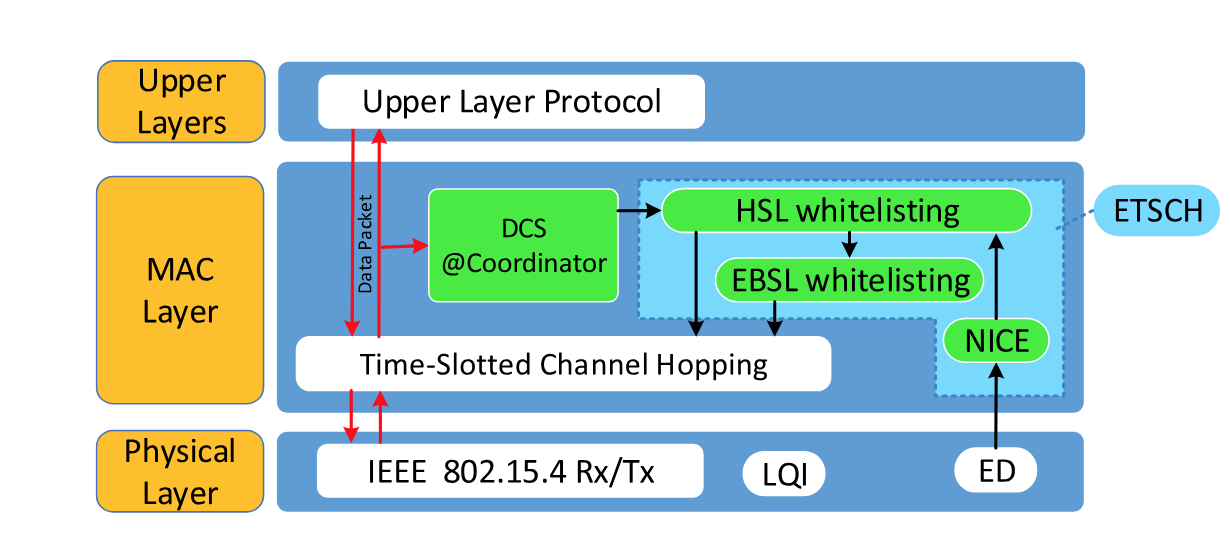
\includegraphics[height=6.5cm,width=7.8cm,scale=.30]{mac.png}
                    
                    \caption{Figure 1: ETSCH+DCS components in the coordinator node.}
                    \label{fig:macp}
              \end{minipage}
             \hspace{0.5cm}
              \begin{minipage}[white]{0.44\linewidth}
                    \centering
                    
                    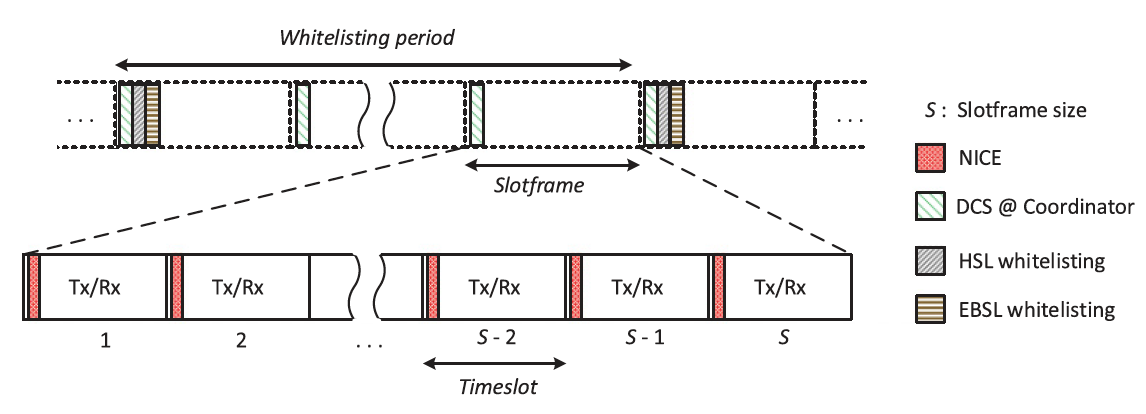
\includegraphics[height=6.5cm,width=12cm, scale=.30]{whitelisting.png}
                    \hspace{3cm}
                    \caption{Figure 2: ETSCH components within TSCH }
                    \label{fig:white}
              \end{minipage}
\end{minipage}
\\\\
As Figure 1 shows, NICE runs in parallel with TSCH on the MAC layer of the coordinator to extract
the quality of all available channels. NICE uses the Energy Detections (EDs) introduced in the protocol to measure
the quality of each frequency channel. An ED is an estimate of the received signal power within
the bandwidth of a channel and takes eight symbol periods.
}
\headerbox{Experiment}{name=experiment, column=1,span =2, below=background}
{Packet Reception Ratio (PRR)
is the number of packets that are successfully received at the receiver node over the total number
of packets transmitted by the sender node, extracted from the experiments. This metric reflects the
quality of the links. The length of burst packet losses is the number of consecutive packets losses
over a link and shows the time duration of link level disconnections. This metric is important for
many applications to avoid long disconnections, as they required continuity of correct service over
time. Figure 3 shows the average of achieved PRR of all links in the network for different mechanisms
and interference scenarios. Both versions of ETSCH provide better PRR on average in comparison
to TSCH and ATSCH when the network experiences dynamic interference. This shows the effect
of highly adaptive channel quality estimation that is realized by NICE, which selects the best
quality channels for hopping. Table 1 considers four interference scenarios in our experiments as follows: high, medium, low, and no interference and observes the behavior of Noise Generators (NGs) at each level of interference. In the no interference scenario, we run the experiments without any controlled
noise generator to see how the cost of periodic Hopping Sequence List (HSL) changes.\\

   \begin{minipage}[interference]{0.99\linewidth}            
    \begin{minipage}[redgraph]{0.45\linewidth}
    \hspace{1.5cm}
    \caption{Table 1: Interference Scenarios and Behavior \label{interference}}\\
    \\
                    \centering
                    \begin{tabular}{ |p{5.2cm}||p{5.2cm}| }
 \hline
 \multicolumn{2}{|c|}{Interference Scenarios} \\
 \hline
 \emph{Scenario} & \emph{Behavior of NG(s)} \\
 \hline
 No interference   & no controlled NG    \\
 \hline
 Low interference &  noise on 2 channels (1 NG), hop every 20s to new channels  \\
 \hline
 Medium interference & noise on 6 channels (3 NGs), hop every 20s to new channels\\
 \hline
 High interference    & noise on 6 channels (3 NGs), hop every 5s to new channels\\
 \hline
\end{tabular}
                    \label{fig:interference}
              \end{minipage}
             \hspace{1cm}
             \begin{minipage}[redgraph]{0.59\linewidth}
                    \centering
                    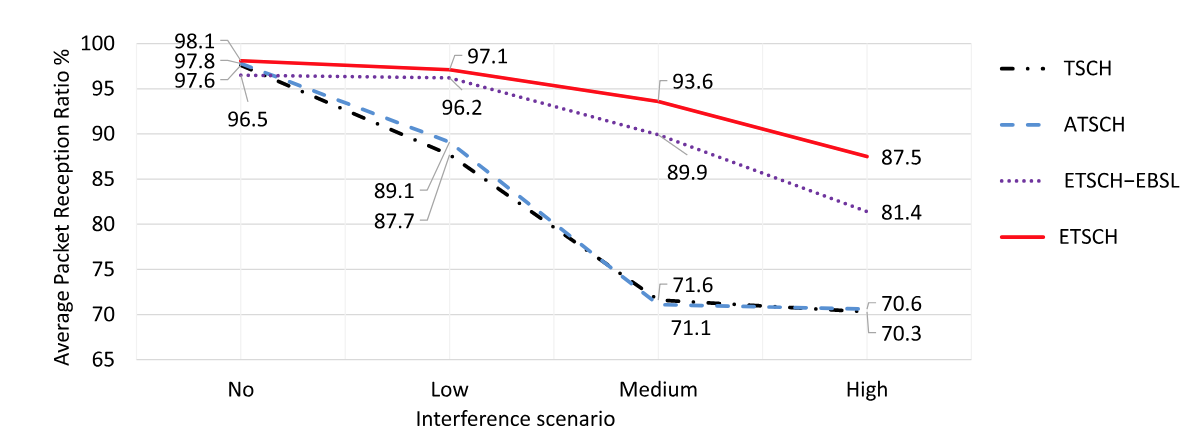
\includegraphics[height=6.5cm,width=7.8cm]{redgraph.png}
                    
                    \caption{Figure 3: Avg. PRR of different interference scenarios.}
                    \label{fig:red}
              \end{minipage}
\end{minipage}
\\\\

As depicted in Figure 3, ATSCH performs almost the same as basic
TSCH. There are two reasons for these results: (1) The rate of channel samplings by ATSCH is
much lower than for ETSCH. Therefore, it can only deal with very low dynamic interference, and
it cannot detect and follow the highly dynamic interference (that exists in in-vehicle networks).
This leads to increasing packet losses when noisy channels are also selected to be used in the HSL.
(2) ATSCH does all the samplings in one timeslot every slotframe. Our NICE technique spreads
channel samplings over a slotframe, and therefore it can detect noisy channels better.
Figure 3 also shows that using an EBSL to disseminate EBs improves the PRR of ETSCH compared
to ETSCH–EBSL in all the interference scenarios. This is because it reduces the possibility
of EB losses and accordingly, HSL mismatches between the coordinator and nodes. 
}
\headerbox{Conclusion}{name=conclusion, column=1, span=2, below=experiment}
{The results of the centralized and distributed channel quality estimation
techniques are used to assign a quality factor to each channel. Using these qualities, channels with
better qualities are periodically selected as the hopping sequence list of TSCH. ETSCH+DCS also
uses a small secondary hopping sequence list (EBSL), that consists of the best quality channels, to
disseminate periodic EBs. These EBs contain control information of the network such as the HSL.
Only one field of the EBSL is updated per period, and thus the rate of EB losses in the network
is reduced compared to using the regular HSL for broadcasting EBs. Experimental and simulation
results show that ETSCH with NICE and EBSL provides higher packet reception ratios and lower
length of burst packet losses compared to the plain TSCH protocol and another related work called
ATSCH. Experiments also show that the DCS technique can detect existing interference in parts
of the network that is not detectable by the centralized NICE technique, and thus it increases the
PRR in those scenarios.}

\headerbox{References}{name=references, column=1, span=2, below=conclusion}
{
- Kannan Srinivasan, Maria A. Kazandjieva, Saatvik Agarwal, and Philip Levis. 2008. The beta-factor-factor: Measuring
wireless link burstiness. In Proceedings of the 6th ACM Conference on Embedded Network Sensor Systems (SenSys’08).
ACM, New York, NY, 29–42. DOI:http://dx.doi.org/10.1145/1460412.1460416

- X. Vilajosana, Q. Wang, F. Chraim, T. Watteyne, T. Chang, and K. S. J. Pister. 2014. A realistic energy consumption
model for TSCH networks. IEEE Sens. J. 14, 2 (Feb. 2014), 482–489. DOI:http://dx.doi.org/10.1109/JSEN.2013.2285411




}
\end{poster}
\end{document}

